\documentclass[11pt,a4paper]{article}
\usepackage[italian]{babel}
\newcommand{\nomeprop}{Proposizione}
\newcommand{\nomelemma}{Lemma}
\newcommand{\nomeoss}{Osservazione}
% voci della bibliografia: numero dell'edizione e data di consultazione
\newcommand{\edizione}[2]{#1\textsuperscript{a} ed.}
\newcommand{\consultato}{consultato nell'ottobre 2026}
% ---------------------------------------------------------------------------
%  Preambolo comune alle due versioni della nota.
%  Il file principale carica babel con la lingua e definisce \nomeprop,
%  \nomelemma e \nomeoss prima di includere questo file.
% ---------------------------------------------------------------------------
\usepackage[T1]{fontenc}
\usepackage[utf8]{inputenc}

\usepackage{lmodern}
\usepackage{textcomp}
\usepackage{microtype}

\usepackage[a4paper,top=2.7cm,bottom=2.9cm,left=2.9cm,right=2.9cm]{geometry}

\usepackage{amsmath}
\usepackage{amssymb}
\usepackage{amsthm}
\usepackage{mathtools}
\usepackage{graphicx}
\usepackage{xcolor}
\usepackage{booktabs}
\usepackage{array}
\usepackage{enumitem}
\usepackage{caption}
\usepackage{titlesec}
\usepackage[hidelinks]{hyperref}

% --- tavolozza, la stessa dell'edizione integrale ----------------------------
\definecolor{inchiostro}{HTML}{1B1F23}
\definecolor{blunotte}{HTML}{1F4E79}
\definecolor{rossoterra}{HTML}{B3352B}
\definecolor{verdesalvia}{HTML}{2A7F62}
\definecolor{grigiocarta}{HTML}{F4F5F7}
\definecolor{grigiotratto}{HTML}{C8CCD2}
\definecolor{grigiotesto}{HTML}{6B7280}

\color{inchiostro}

% --- titolazione ------------------------------------------------------------
\titleformat{\section}
  {\normalfont\sffamily\Large\bfseries\color{blunotte}}{\thesection}{0.7em}{}
\titleformat{\subsection}
  {\normalfont\sffamily\large\bfseries\color{inchiostro}}
  {\thesubsection}{0.6em}{}
\titleformat{\paragraph}[runin]
  {\normalfont\sffamily\bfseries\color{inchiostro}}{}{0pt}{}

\captionsetup{font=small,labelfont={sf,bf,color=blunotte},
              labelsep=period,width=0.92\linewidth}

\graphicspath{{../figures/}}

% --- enunciati ----------------------------------------------------------------
\theoremstyle{plain}
\newtheorem{prop}{\nomeprop}[section]
\newtheorem{lemma}[prop]{\nomelemma}
\theoremstyle{remark}
\newtheorem*{oss}{\nomeoss}

% --- riferimenti alle righe dei quaderni --------------------------------------
% \mbox: un riferimento non va mai spezzato a fine riga
\newcommand{\riga}[2]{\mbox{\texttt{#1}\,\#{}#2}}
\newcommand{\righe}[3]{\mbox{\texttt{#1}\,\#{}#2--#3}}

% --- notazione ----------------------------------------------------------------
\newcommand{\dd}{\mathrm{d}}
\newcommand{\ee}{\mathrm{e}}
\newcommand{\ii}{\mathrm{i}}
\DeclareMathOperator{\sgn}{sgn}
\DeclareMathOperator{\artanh}{artanh}
\DeclareMathOperator{\gd}{gd}
\DeclareMathOperator{\sech}{sech}
\DeclareMathOperator{\sinc}{sinc}
\DeclareMathOperator{\Real}{Re}
\DeclareMathOperator{\Imag}{Im}

\setlength{\emergencystretch}{2em}

\hypersetup{pdftitle={I quaderni Derive, 2009–2011: osservazioni da un taccuino di calcolo simbolico},pdfauthor={Francesco Messina},pdflang={it}}

\title{\sffamily\bfseries\color{blunotte}I quaderni Derive, 2009--2011\\[6pt]\large\mdseries\color{inchiostro}Osservazioni da un taccuino di calcolo simbolico}
\author{Francesco Messina}
\date{Ottobre 2026}

\begin{document}
\maketitle

\begin{abstract}
Fra il 2009 e il 2011 l'autore ha usato il sistema di calcolo simbolico
Derive come taccuino per esperimenti di matematica: ventitr\'e file,
$792$ espressioni. Il programma non \`e pi\`u in uso e i file sono stati
recuperati decodificandone il formato binario. Questa nota non presenta
teoremi nuovi. Raccoglie sette temi in cui gli esperimenti toccano matematica
nota --- la tangente del semiangolo e la frazione continua di Euler per $\ee$,
l'equazione $a!\,b!=c!$, il teorema della media per l'equazione di
Helmholtz, la trasformata di Hilbert, la dequantizzazione di Maslov,
l'accelerazione di una successione per $\ee$, la delta di Dirac fuori
dall'asse reale --- e per ciascuno dice che cosa il quaderno ha visto, che
cosa \`e vero, che cosa \`e gi\`a noto e che cosa resta aperto. Per una
catena di uguaglianze fra fattoriali, vera nei primi quattro casi, si dimostra
che non si richiude pi\`u. Ogni valore numerico citato \`e verificato da
uno script incluso nel repository.

\end{abstract}

\section{Introduzione}
\label{sec:intro}

Fra l'aprile del 2009 e il gennaio del 2011 l'autore ha usato \emph{Derive
for Windows}, il sistema di calcolo simbolico della Texas Instruments, come
un taccuino: si scrive un'espressione, si chiede al programma di
semplificarla, risolverla, derivarla o farne il limite, si cambia un
parametro e si guarda che cosa succede. Ne sono rimasti ventitr\'e file
\texttt{.dfw} con $792$ espressioni. \`E matematica sperimentale nel senso
di~\cite{borwein2008}: raramente una dimostrazione, spesso una regolarit\`a
intravista, a volte un errore.

Derive \`e stato ritirato dal commercio nel 2007 e non \`e pi\`u mantenuto; i
suoi file non si aprono con i programmi di calcolo attuali, ma conservano le
espressioni come testo. Il recupero, che
consiste nel decodificare il formato, tradurre le espressioni in notazione
matematica e verificarle numericamente, \`e descritto
nell'appendice~\ref{app:recupero}. Il risultato completo \`e un'edizione
integrale di oltre duecento pagine, in cui ogni espressione \`e riprodotta e
commentata.

Questa nota \`e un'altra cosa: una scelta per temi, pensata per un lettore
matematico. Ogni sezione dice che cosa fa il quaderno, enuncia in forma
pulita quello che c'\`e di vero, lo dimostra o ne abbozza la dimostrazione,
lo colloca nella letteratura e dice che cosa resta aperto. Nessun risultato
\`e presentato come nuovo. L'unica dimostrazione che non abbiamo trovato in
letteratura, quella della sezione~\ref{sec:fattoriali}, \`e elementare.

In sintesi:
\begin{itemize}[leftmargin=1.4em,itemsep=1pt]
  \item la sezione~\ref{sec:semiangolo} ricostruisce l'idea che attraversa
        cinque quaderni, scrivere l'esponenziale con la tangente del
        semiangolo, e la segue fino a Euler, Lambert, Pad\'e e alla
        trasformazione bilineare dei filtri numerici;
  \item la sezione~\ref{sec:fattoriali} spiega una regolarit\`a fra
        fattoriali che dura quattro passi e dimostra che non si ripete;
  \item le sezioni~\ref{sec:media}, \ref{sec:cosinc}, \ref{sec:gradini}
        e~\ref{sec:e} riconducono altri quattro quaderni a fatti noti: il
        teorema della media per l'equazione di Helmholtz, la trasformata di
        Hilbert, la dequantizzazione di Maslov, l'eliminazione dei termini
        dispari dell'errore;
  \item la sezione~\ref{sec:delta} discute un calcolo con un'interpretazione
        che non regge, e lascia aperta la domanda;
  \item la sezione~\ref{sec:mezzo} raccoglie la formula preferita dei
        quaderni, le sue varianti e la sua forma generale;
  \item la sezione~\ref{sec:breve} riassume gli altri quaderni, la
        sezione~\ref{sec:refusi} gli errori.
\end{itemize}

\paragraph{Come si leggono i riferimenti.}
La scrittura \riga{factor.dfw}{4} indica l'espressione numero~4 del file
\texttt{factor.dfw}, con la numerazione di Derive; \righe{gauss.dfw}{1}{5}
indica un intervallo di espressioni. L'edizione integrale le riproduce tutte
con la stessa numerazione.

\paragraph{Verifica.}
Ogni valore numerico citato nella nota \`e ricalcolato da uno script incluso
nel repository, \texttt{verifica\_nota.py}, con \texttt{mpmath} a sessanta
cifre; un secondo script controlla che ogni decimale presente nel testo sia
fra quelli verificati, e che la versione italiana e quella inglese riportino
gli stessi numeri, gli stessi riferimenti e le stesse citazioni.

\section{L'esponenziale e la tangente del semiangolo}
\label{sec:semiangolo}

Cinque quaderni --- \texttt{gauss}, \texttt{atan}, \texttt{cosinc},
\texttt{delta} e \texttt{mate} --- contengono pezzi della stessa idea:
scrivere l'esponenziale come funzione razionale della tangente dell'angolo
met\`a. Nessuno la enuncia per intero. Messa insieme, porta a una serie di
risultati classici: la parametrizzazione razionale del cerchio, la funzione
gudermanniana, la frazione continua di Euler per $\ee$, gli approssimanti di
Pad\'e e la trasformazione bilineare dei filtri numerici. Niente di questo
\`e nuovo; vale la pena raccontarlo perch\'e \`e il filo che tiene insieme il
materiale pi\`u interessante della raccolta.

\subsection{Il cerchio e l'asse immaginario}

\begin{prop}\label{prop:semiangolo}
Per $|t|<\pi$, posto $u=\tan(t/2)$,
\begin{equation}\label{eq:cayley}
  \ee^{\ii t}=\frac{1+\ii u}{1-\ii u}=\frac{(1+\ii u)^2}{1+u^2}
  =\sgn(1+\ii u)^2 ,
\end{equation}
dove $\sgn z=z/|z|$. Per ogni $s$ reale, posto $\tau=\tanh(s/2)$,
\begin{equation}\label{eq:tanh}
  \ee^{s}=\frac{1+\tau}{1-\tau},
  \qquad\text{cio\`e}\qquad
  s=\ln\frac{1+\tau}{1-\tau}=2\artanh\tau .
\end{equation}
\end{prop}

\begin{proof}
Poich\'e $\cos(t/2)>0$, si ha $1\pm\ii u=\ee^{\pm\ii t/2}/\cos(t/2)$: il
rapporto vale $\ee^{\ii t}$, e da $1+\ii u=|1+\ii u|\,\ee^{\ii t/2}$ segue
l'ultima forma. Per la seconda parte,
$(1+\tau)/(1-\tau)=(\cosh\frac s2+\sinh\frac s2)/(\cosh\frac s2-\sinh\frac s2)
=\ee^{s/2}/\ee^{-s/2}$.
\end{proof}

Separando parte reale e immaginaria della \eqref{eq:cayley} si ottiene
$\cos t=(1-u^2)/(1+u^2)$ e $\sin t=2u/(1+u^2)$: la parametrizzazione
razionale del cerchio, che per $u=q/p$ razionale d\`a le terne pitagoriche
$(p^2-q^2,\,2pq,\,p^2+q^2)$. Geometricamente $\ee^{\ii t}$ \`e il punto in
cui la retta per $-1$ e per $\ii u$ taglia di nuovo il cerchio: una
proiezione stereografica dal punto $-1$ (figura~\ref{fig:nota_semiangolo},
a sinistra).

La seconda forma della \eqref{eq:cayley} \`e quella che il quaderno scrive in
\righe{gauss.dfw}{1}{4}, osservando anche che $1+u^2$ \`e la derivata di
$2u$ rispetto a $t$: l'esponenziale immaginario come quadrato diviso per una
derivata. La terza forma, con $t$ al posto di $t/2$, compare in
\righe{cosinc.dfw}{1}{3} e in \riga{delta.dfw}{41}.

La \eqref{eq:tanh} \`e la \eqref{eq:cayley} letta sull'asse immaginario:
poich\'e $\tan(\ii y)=\ii\tanh y$, ponendo $t=-\ii s$ si ha
$1\pm\ii u=1\pm\tanh(s/2)$. Il cerchio si apre nella semiretta positiva:
$\tau$ percorre $(-1,1)$ e $\ee^{s}$ percorre $(0,\infty)$. I quaderni
arrivano a questa formula da due lati.

\paragraph{La gaussiana.}
\riga{gauss.dfw}{5} pone $t=\ii x^2$ nella \eqref{eq:cayley} e trova la
gaussiana:
\[
  \ee^{-x^2}=\frac{1-\tanh(x^2/2)}{1+\tanh(x^2/2)} ,
\]
cio\`e la \eqref{eq:tanh} con $s=-x^2$. Il quaderno vorrebbe poi arrivare
alla funzione degli errori integrando $\sgn(1+\ii u)$
(\righe{gauss.dfw}{6}{14}), e la proposizione spiega perch\'e la strada non
porta lontano: sull'asse reale l'informazione sta nella \emph{fase} di
$1+\ii u$, il cui modulo vale $1/\cos(t/2)$; sull'asse immaginario
$1+\ii u=1-\tanh(x^2/2)$ \`e reale e positivo, la sua funzione segno vale
identicamente $1$, e la gaussiana sta tutta nel \emph{modulo}.

\paragraph{L'arcotangente di argomento immaginario.}
\righe{atan.dfw}{1}{14} parte da $\ee^{\ii\arctan x}=(1+\ii x)/\sqrt{1+x^2}$,
che \`e la \eqref{eq:cayley} nella forma $\sgn(1+\ii u)=\ee^{\ii t/2}$, e
sostituisce $x$ con $\ii x$. Per $|x|<1$ vale $\arctan(\ii x)=\ii\artanh x$, e
la riga \#2 trova
\[
  \ee^{\ii\arctan(\ii x)}=\sqrt{\frac{1-x}{1+x}}=\ee^{-\artanh x},
\]
che \`e la \eqref{eq:tanh} con $\tau=x$. Le righe \#3 e \#4 raggiungono il
punto di diramazione $x=1$ ($\arctan\ii=\ii\infty$), e le righe da \#5 a \#14
ricostruiscono la forma logaritmica
$\ii\arctan(\ii x)=\ln(1-x)-\tfrac12\ln(1-x^2)=-\artanh x$, tenendo conto
correttamente dei rami del logaritmo.

\paragraph{La gudermanniana.}
Se lo stesso numero $\tau$ fa da tangente del semiangolo sia per un angolo
circolare $\theta$ sia per un argomento iperbolico $s$, cio\`e se
$\tan(\theta/2)=\tanh(s/2)$, la proposizione d\`a senza passare per i numeri
complessi
\[
  \cos\theta=\frac{1-\tau^2}{1+\tau^2}=\sech s,\qquad
  \sin\theta=\frac{2\tau}{1+\tau^2}=\tanh s,\qquad
  \tan\theta=\frac{2\tau}{1-\tau^2}=\sinh s .
\]
La funzione $s\mapsto\theta=\gd s=2\arctan\bigl(\tanh(s/2)\bigr)$ \`e la
gudermanniana. Le righe \righe{mate.dfw}{111}{122} cercano, per ciascuna
funzione iperbolica, una funzione circolare con lo stesso valore:
$\tanh x=\tan(kx)$, $\sinh x=\sin(kx)$ e cos\`i via. Le risposte di Derive
sono corrette caso per caso --- per esempio $kx=\arctan(\tanh x)$, che vale
$\tfrac12\gd(2x)$ --- ma la risposta sistematica \`e la gudermanniana:
$\tan(\gd x)=\sinh x$, $\sin(\gd x)=\tanh x$, $\cos(\gd x)=\sech x$.

\begin{figure}[t]
  \centering
  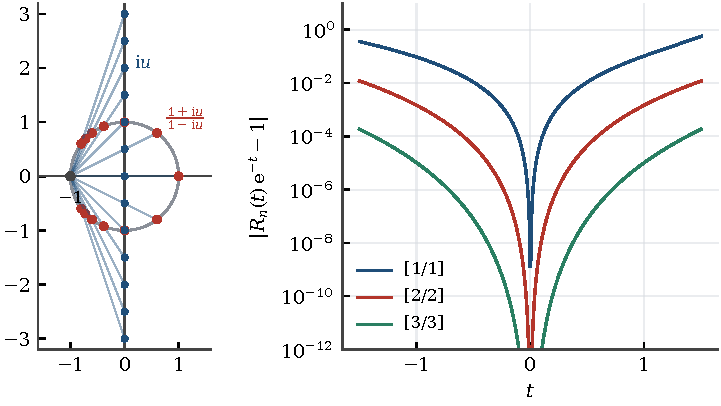
\includegraphics[width=\linewidth]{nota_semiangolo}
  \caption{A sinistra, la proiezione stereografica dal punto $-1$: la retta
  per $-1$ e per $\ii u$ taglia il cerchio in $(1+\ii u)/(1-\ii u)=\ee^{\ii t}$,
  per $u=-3,-2{,}5,\dots,3$. A destra, l'errore relativo degli approssimanti
  di Pad\'e diagonali $R_1$, $R_2$, $R_3$ di $\ee^{t}$, ottenuti troncando la
  frazione continua di Lambert.}
  \label{fig:nota_semiangolo}
\end{figure}

\subsection{Il numero \texorpdfstring{$\ee$}{e} e le frazioni continue}

Con $s=1$ la \eqref{eq:tanh} d\`a
\[
  \ee=\frac{1+\tanh\frac12}{1-\tanh\frac12},
  \qquad
  \tanh\tfrac12=\frac{\ee-1}{\ee+1}=0{,}46211715\dots
\]
Questo numero ha una frazione continua celebre, trovata da Euler nel
1737~\cite{eulero1744}:
\[
  \frac{\ee-1}{\ee+1}
  =\cfrac{1}{2+\cfrac{1}{6+\cfrac{1}{10+\cfrac{1}{14+\dotsb}}}}
  =[0;\,2,6,10,14,\dots],
\]
con i quozienti parziali in progressione aritmetica. Pi\`u in generale, per
ogni intero positivo $n$,
\[
  \tanh\frac1n=[0;\,n,3n,5n,\dots].
\]
Entrambe discendono dalla frazione continua di Lambert~\cite{lambert1768}
\[
  \tanh x=\cfrac{x}{1+\cfrac{x^2}{3+\cfrac{x^2}{5+\dotsb}}} ,
\]
ponendo $x=1/n$ e liberando i denominatori. Lambert la us\`o per dimostrare
che $\tanh x$, e quindi $\ee^{2x}=(1+\tanh x)/(1-\tanh x)$, \`e irrazionale
per ogni $x$ razionale non nullo; la frazione analoga per $\tan x$, con
$\tan(\pi/4)=1$, d\`a l'irrazionalit\`a di $\pi$. Per $\ee$, dunque, la
formula $\ee^{s}=(1+\tau)/(1-\tau)$ \`e proprio un passaggio della prima
dimostrazione di irrazionalit\`a; per $\pi$ ne serve la versione circolare,
con $\tan$ al posto di $\tanh$. I quaderni non arrivano fin qui, ma \`e l\`i
che la loro idea conduce.

\subsection{Troncare: gli approssimanti di Pad\'e}

Troncando la frazione di Lambert per $\tanh(t/2)$ e sostituendo nella
\eqref{eq:tanh} si ottiene, al primo, al secondo e al terzo livello,
\[
  R_1(t)=\frac{2+t}{2-t},\qquad
  R_2(t)=\frac{12+6t+t^2}{12-6t+t^2},\qquad
  R_3(t)=\frac{120+60t+12t^2+t^3}{120-60t+12t^2-t^3}.
\]
Sono gli approssimanti di Pad\'e diagonali $[n/n]$ di $\ee^{t}$: le funzioni
razionali con numeratore e denominatore di grado $n$ che coincidono con
$\ee^{t}$ fino all'ordine $t^{2n}$; per esempio
$R_1(t)-\ee^{t}=t^3/12+O(t^4)$. Che i convergenti della frazione di Lambert
diano esattamente la diagonale della tavola di Pad\'e dell'esponenziale \`e
un fatto generale~\cite{baker1996}; qui lo abbiamo verificato per
$n\le3$. Dalla formula esatta gli approssimanti ereditano due propriet\`a:
$R_n(-t)=1/R_n(t)$, come $\ee^{t}$, e $|R_n(\ii\omega)|=1$ per ogni $\omega$
reale, perch\'e numeratore e denominatore sono coniugati sull'asse
immaginario. Mandano cio\`e l'asse immaginario sul cerchio unitario,
esattamente come $\ee^{\ii\omega}$; anzi $R_1(\ii\omega)$ \`e la
\eqref{eq:cayley} con $u=\omega/2$. L'errore relativo dei primi tre
approssimanti \`e nella figura~\ref{fig:nota_semiangolo}, a destra.

\subsection{Un'applicazione: i filtri numerici}

Un filtro analogico con funzione di trasferimento $H(s)$ si trasforma in un
filtro numerico, con passo di campionamento $T$, esprimendo $s$ attraverso
$z=\ee^{sT}$. Per la \eqref{eq:tanh} la relazione esatta \`e
\[
  \frac{z-1}{z+1}=\tanh\frac{sT}{2},
  \qquad\text{cio\`e}\qquad
  s=\frac2T\artanh\frac{z-1}{z+1},
\]
che non \`e razionale in $z$. La trasformazione bilineare (di Tustin)
sostituisce $\tanh(sT/2)$ con la sua prima approssimazione $sT/2$:
\[
  s\;\mapsto\;\frac2T\,\frac{z-1}{z+1},
  \qquad\text{cio\`e}\qquad
  z=\frac{1+sT/2}{1-sT/2}=R_1(sT).
\]
Poich\'e $|R_1(\ii\Omega T)|=1$ e $|R_1(s)|<1$ per $\Real s<0$, l'asse
immaginario va sul cerchio unitario e il semipiano sinistro nel disco: un
filtro stabile resta stabile. Il prezzo si paga in frequenza: sul cerchio
$z=\ee^{\ii\omega T}$, e la \eqref{eq:cayley} d\`a
$(z-1)/(z+1)=\ii\tan(\omega T/2)$, quindi alla frequenza numerica $\omega$
corrisponde la frequenza analogica
\[
  \Omega=\frac2T\tan\frac{\omega T}{2}.
\]
\`E la distorsione delle frequenze della trasformazione bilineare; il rimedio
abituale, \emph{precompensare} le frequenze critiche con questa stessa
formula, si trova nei manuali di elaborazione numerica dei
segnali~\cite{oppenheim2010}. Se il filtro elimina-banda progettato in
\texttt{notch.dfw} venisse realizzato in forma numerica, la sua pulsazione di
antirisonanza andrebbe precompensata proprio cos\`i: la tangente del
semiangolo di \texttt{gauss.dfw} \`e la stessa dell'ingegnere.

Lo stesso schema compare in relativit\`a ristretta: se $\beta=\tanh\eta$ \`e
la velocit\`a in unit\`a di $c$ e $\eta$ la rapidit\`a, il fattore Doppler
\`e $\ee^{\eta}=\sqrt{(1+\beta)/(1-\beta)}=(1+\tanh\frac\eta2)/(1-\tanh\frac\eta2)$.

\paragraph{Che cosa resta aperto.}
Nulla, sul piano matematico: tutto ci\`o che compare in questa sezione \`e
classico. Quello che i quaderni aggiungono \`e l'aver percorso, senza saperlo,
un tratto della stessa strada da cinque lati diversi.

\section{Una catena di fattoriali che si spezza}
\label{sec:fattoriali}

\section{La media e il punto medio}
\label{sec:media}

L'ultimo quaderno della raccolta, \texttt{Trasformata T.dfw} (gennaio 2011),
applica a quattordici funzioni lo stesso operatore,
\[
  T[f](t)=\frac{\dfrac1t\displaystyle\int_0^t f(x)\,\dd x}{f(t/2)},
\]
cio\`e il rapporto fra la media di $f$ sull'intervallo $[0,t]$ e il valore
di $f$ nel punto medio. Per una funzione affine il rapporto vale $1$. Le
righe \righe{Trasformata T.dfw}{3}{8} trovano
\begin{gather*}
  T[\sin]=T[\cos]=T[\ee^{\ii x}]=\frac{\sin(t/2)}{t/2},\qquad
  T[\ee^{2\pi\ii x}]=\frac{\sin(\pi t)}{\pi t},\\
  T[\ee^{x}]=\frac{\sinh(t/2)}{t/2},\qquad
  T[x^n]=\frac{2^n}{n+1}.
\end{gather*}
Tre funzioni diverse danno lo stesso seno cardinale, e il quaderno lo
registra senza commento. La ragione \`e questa.

\begin{prop}\label{prop:media}
Sia $f$ di classe $C^2$ con $f''=\mu^2 f$ per una costante complessa $\mu$.
Allora, per ogni intervallo $[c-h,c+h]$ del dominio,
\[
  \frac1{2h}\int_{c-h}^{c+h}f(x)\,\dd x=f(c)\,\frac{\sinh(\mu h)}{\mu h},
\]
dove il fattore vale $1$ per $\mu=0$. In particolare, dove $f(t/2)\neq0$,
$T[f](t)=\sinh(\mu t/2)/(\mu t/2)$: il seno cardinale $\sin(t/2)/(t/2)$ per
ogni soluzione di $f''=-f$, il suo analogo iperbolico per ogni soluzione di
$f''=f$.
\end{prop}

\begin{proof}
Se $\mu\neq0$, $f=A\ee^{\mu x}+B\ee^{-\mu x}$. La media di $\ee^{\mu x}$ su
$[c-h,c+h]$ vale $\ee^{\mu c}(\ee^{\mu h}-\ee^{-\mu h})/(2\mu h)
=\ee^{\mu c}\sinh(\mu h)/(\mu h)$; il fattore \`e pari in $\mu$, quindi vale
lo stesso per $\ee^{-\mu x}$, e si conclude per linearit\`a. Se $\mu=0$, $f$
\`e affine e la media coincide con il valore nel punto medio.
\end{proof}

\begin{oss}
Vale anche il viceversa, nella forma seguente: se $f\in C^2$ e la media di
$f$ su $[c-h,c+h]$ vale $\varphi(h)\,f(c)$ per ogni $c$, con $\varphi$
indipendente da $c$, allora $f''=\lambda f$ per una costante $\lambda$.
Infatti la media vale $f(c)+f''(c)h^2/6+o(h^2)$; scelto $c_0$ con
$f(c_0)\neq0$, ne segue che $(\varphi(h)-1)/h^2$ ha un limite $L$, e allora
$f''(c)=6L\,f(c)$ per ogni $c$. Le funzioni per cui il rapporto fra media e
valore centrale dipende solo dall'ampiezza dell'intervallo sono dunque
esattamente le soluzioni di $f''=\lambda f$: \`e questa la struttura che le
righe da \#3 a \#7 mettono in luce.
\end{oss}

Le potenze sono un caso diverso: $T[x^n]$ \`e costante per omogeneit\`a, e lo
stesso conto d\`a $2^\alpha/(\alpha+1)$ per ogni $f(x)=x^\alpha$ con
$\alpha>-1$. Per le altre funzioni del quaderno --- logaritmi, arcotangente,
arcoseno, gaussiana, seno integrale --- $T[f]$ dipende da $t$ senza una
struttura altrettanto semplice.

\paragraph{Il contesto.}
La proposizione \`e il caso unidimensionale del teorema della media per
l'equazione di Helmholtz. Se $\Delta u+k^2u=0$ in un intorno della palla
chiusa di centro $x$ e raggio $r$ in $\mathbb{R}^n$, la media $M(r)$ di $u$
sulla sfera di raggio $r$ soddisfa
$M''+\frac{n-1}{r}M'+k^2M=0$, con $M(0)=u(x)$ e $M'(0)=0$ (l'equazione di
Darboux per le medie sferiche~\cite{john1955}), e quindi
\[
  M(r)=u(x)\,\Gamma\Bigl(\frac n2\Bigr)\Bigl(\frac{2}{kr}\Bigr)^{n/2-1}
  J_{n/2-1}(kr).
\]
Per $n=1$ la ``sfera'' \`e la coppia di punti $c\pm r$ e $M(r)=u(c)\cos(kr)$;
mediando sul raggio si ottiene la media sull'intervallo,
$u(c)\sin(kr)/(kr)$, che \`e la proposizione con $\mu=\ii k$. Per $n=3$ si
ottiene $M(r)=u(x)\sin(kr)/(kr)$: la media su un segmento in dimensione uno
ha lo stesso nucleo della media su una sfera in dimensione tre.

\section{Il seno cardinale e il suo gemello}
\label{sec:cosinc}

\section{Gradini fatti di logaritmi}
\label{sec:gradini}

Le righe \righe{mate.dfw}{77}{84} costruiscono il gradino di Heaviside $H$,
la funzione segno e alcune onde quadre usando soltanto esponenziali,
logaritmi e valori assoluti. La costruzione \`e esatta, e il motivo \`e un
lemma elementare.

\begin{lemma}\label{lemma:massimo}
Per $a,b$ reali,
$\dfrac{|a-b|+|a+b|}{2}=\max\bigl(|a|,|b|\bigr)$.
\end{lemma}

\begin{proof}
Se $|a|\ge|b|$, i numeri $a-b$ e $a+b$ hanno entrambi il segno di $a$ (o sono
nulli), quindi $|a-b|+|a+b|=|2a|$. Il caso $|b|\ge|a|$ \`e simmetrico.
\end{proof}

Con $a=\ee^{x}$ e $b=1$ il lemma d\`a
$\ln\bigl((|\ee^x-1|+|\ee^x+1|)/2\bigr)=\ln\max(\ee^x,1)=\max(x,0)$, e quindi,
per $x\neq0$,
\[
  \frac{1}{x}\ln\frac{|\ee^x-1|+|\ee^x+1|}{2}=\frac{\max(x,0)}{x}=H(x),
  \qquad
  \frac{2}{x}\ln\frac{|\ee^x-1|+|\ee^x+1|}{2}-1=\sgn x ,
\]
che sono le righe \#77 e \#81 (la \#80 ottiene il segno con $\ee^{2x}$ al
posto di $\ee^{x}$). Componendo con $\sin\pi x$ si ottengono le onde quadre
delle righe \#82--\#84. Logaritmo ed esponenziale sono a rigore una
deviazione, perch\'e $H(x)=\max(x,0)/x=(x+|x|)/(2x)$; quello che la
costruzione mette davvero in luce \`e che il logaritmo trasforma il massimo
di due esponenziali nel massimo degli esponenti,
$\ln\max(\ee^{a},\ee^{b})=\max(a,b)$.

\paragraph{Il logaritmo del coseno iperbolico.}
La versione di febbraio dello stesso quaderno annota
$\ln\cosh x=|x|$ (\righe{mate copia.dfw}{88}{89}). L'uguaglianza \`e solo
asintotica:
\[
  \ln\cosh x=|x|-\ln2+\ln\bigl(1+\ee^{-2|x|}\bigr),
\]
quindi $\ln\cosh x-|x|\to-\ln2$ per $|x|\to\infty$, mentre vicino a zero
$\ln\cosh x\approx x^2/2$. Le due righe stanno in un rapporto preciso con la
costruzione esatta: $\cosh x=(\ee^{x}+\ee^{-x})/2$ \`e la \emph{media} di due
esponenziali, mentre $\ee^{|x|}=\max(\ee^{x},\ee^{-x})$ ne \`e il
\emph{massimo}.

\paragraph{Il contesto.}
Il passaggio dalla media (o dalla somma) al massimo ha un nome. Per ogni
$h>0$
\[
  \max(a,b)\le h\ln\bigl(\ee^{a/h}+\ee^{b/h}\bigr)\le\max(a,b)+h\ln2 ,
\]
quindi per $h\to0$ la somma diventa il massimo e, di conseguenza, il prodotto
diventa la somma. \`E la \emph{dequantizzazione di Maslov}, e l'aritmetica
$(\max,+)$ che ne risulta \`e quella della matematica
tropicale~\cite{litvinov2007}. I valori assoluti di \texttt{mate.dfw}
calcolano il massimo esatto, cio\`e il caso limite $h=0$; il $\ln\cosh$ di
\texttt{mate copia.dfw} \`e il caso $h=1$, con la media al posto della somma.
La stessa coppia ricorre nelle reti neurali come
$\mathrm{softplus}(x)=\ln(1+\ee^{x})$ e $\mathrm{ReLU}(x)=\max(x,0)$: il
gradino dei quaderni \`e $\mathrm{ReLU}(x)/x$.

\paragraph{Quanto vale un gradino nel salto.}
La formula $\max(x,0)/x$ non d\`a alcun valore in $x=0$. Un valore si ottiene
solo scegliendo una famiglia regolare che converga al gradino, e dipende
dalla scelta. La famiglia
\[
  H_h(x)=\frac{h}{x}\ln\frac{1+\ee^{x/h}}{2},
\]
che \`e la costruzione dei quaderni con la media al posto del massimo,
converge a $H$ per $x\neq0$ quando $h\to0$ e ha limite $\tfrac12$ in $x=0$
per ogni $h$: \`e la convenzione usuale $H(0)=\tfrac12$. Ma anche
$\frac12\bigl(1+\tanh(x/h+1)\bigr)$ converge a $H$ per $x\neq0$, e in $x=0$
vale $\frac12(1+\tanh1)=0{,}8808$ per ogni $h$.

Il quaderno \texttt{u(0)-sign(0).dfw} (gennaio 2011) affronta proprio questa
domanda, con quattro numeri e le loro differenze
(\righe{u(0)-sign(0).dfw}{1}{12}). Le righe \#1, \#3, \#5 e \#7
contengono le forme chiuse: un candidato per il gradino,
$u_1=\ln(\ee-1)=0{,}5413$, e uno per il segno, $s_2=\ln\sinh1=0{,}1614$, che
la riga \#3 scrive $\ln\bigl((\ee^2-1)/(2\ee)\bigr)$; le righe \#5 e \#7 portano ciascuno
nell'altra scala con $\sgn=2H-1$, e le righe da \#9 a \#12 confrontano i
risultati. Che la seconda differenza sia esattamente il doppio della prima
discende dalla conversione stessa. Il quaderno non dice da quale famiglia
vengano i due candidati, e non \`e possibile ricostruirlo con certezza;
nessuno dei due coincide con la convenzione simmetrica $H(0)=\tfrac12$,
$\sgn0=0$. Non \`e un errore: senza una famiglia la domanda non ha una
risposta sola.

\paragraph{Che cosa resta aperto.}
Nulla di matematico: la dequantizzazione di Maslov \`e teoria nota, e la
domanda di \texttt{u(0)-sign(0).dfw} non ha una risposta sola.

\section{Due successioni per \texorpdfstring{$\ee$}{e}}
\label{sec:e}

\section{Una delta di Dirac fuori dall'asse reale}
\label{sec:delta}

\section{La formula preferita dei quaderni}
\label{sec:mezzo}

Il quaderno \texttt{mate.dfw} torna una quarantina di volte sulla stessa
identit\`a,
\begin{equation}\label{eq:mezzo}
  \frac{\cos^2x-\cos^2y}{\cos2x-\cos2y}=\frac12 ,
\end{equation}
vera per ogni $x$ e $y$ con $\cos2x\neq\cos2y$, perch\'e $\cos2\theta=2\cos^2\theta-1$
e quindi $\cos2x-\cos2y=2(\cos^2x-\cos^2y)$ (\riga{mate.dfw}{2}). La parte
interessante \`e il modo in cui il quaderno la mette alla prova.

\subsection{Le varianti}

\begin{itemize}[leftmargin=1.4em,itemsep=2pt]
  \item Con i seni il rapporto vale $-\tfrac12$, perch\'e
        $\sin^2\theta=(1-\cos2\theta)/2$ cambia il segno (\riga{mate.dfw}{4});
        con i coseni iperbolici vale di nuovo $\tfrac12$, perch\'e
        $\cosh2\theta=2\cosh^2\theta-1$ ha la stessa forma (\riga{mate.dfw}{3}).
  \item L'identit\`a vale per argomenti complessi qualsiasi: le righe
        \righe{mate.dfw}{19}{31} la provano con $x\pm\ii y$, con $x\pm ky$, con
        $3x+ky$ e $x$, e la riga \#6 la riscrive con gli esponenziali complessi.
  \item Con la formula di triplicazione $\cos3\theta=4\cos^3\theta-3\cos\theta$
        la costante si dimezza ancora (\riga{mate.dfw}{5}):
        \begin{equation}\label{eq:quarto}
          \frac{\cos^3x\,\cos y-\cos^3y\,\cos x}{\cos3x\,\cos y-\cos3y\,\cos x}=\frac14 .
        \end{equation}
        Moltiplicare per l'altro coseno serve a eliminare il termine
        $-3\cos\theta$.
  \item Con due pesi, il rapporto
        $(\cos^2x-k\cos^2y)/(\cos2x-l\cos2y)$ vale $\tfrac12$ per ogni $x$ se e
        solo se $2k\cos^2y=1+l\cos2y$, cio\`e $\cos2y=(1-k)/(k-l)$: \`e la
        relazione che Derive trova in \righe{mate.dfw}{53}{60}.
  \item Infine la \eqref{eq:mezzo} diventa una ``macchina per $\pi$''
        (\righe{mate.dfw}{67}{71}): poich\'e $(1/2)!=\Gamma(3/2)=\sqrt\pi/2$,
        \[
          4\left[\left(\frac{\cos^2x-\cos^2y}{\cos2x-\cos2y}\right)!\,\right]^2=\pi
        \]
        per ogni coppia di angoli.
\end{itemize}

\subsection{La forma generale}

Le costanti $\tfrac12$ e $\tfrac14$ sono i reciproci dei coefficienti
direttivi dei polinomi di Chebyshev $T_2(c)=2c^2-1$ e $T_3(c)=4c^3-3c$, con
$\cos n\theta=T_n(\cos\theta)$. Con due soli angoli il trucco si ferma al terzo
grado: $T_4(c)=8c^4-8c^2+1$ ha due termini di grado inferiore da eliminare, e
una combinazione di due coseni non basta. Con pi\`u angoli, invece, la regola
vale per ogni grado.

\begin{prop}\label{prop:chebyshev}
Siano $n\ge2$, $m=\lfloor n/2\rfloor+1$, $x_1,\dots,x_m$ angoli e
$c_i=\cos x_i$. Allora
\[
  \det\bigl[\cos nx_i,\ c_i^{\,n-2},\ c_i^{\,n-4},\ \dots,\ c_i^{\,n-2m+2}\bigr]
  =2^{n-1}\det\bigl[c_i^{\,n},\ c_i^{\,n-2},\ c_i^{\,n-4},\ \dots,\ c_i^{\,n-2m+2}\bigr],
\]
dove ogni scrittura indica la matrice $m\times m$ le cui righe sono indicizzate
da $i$. Il determinante a destra \`e diverso da zero se i $c_i^2$ sono distinti
e, per $n$ dispari, non nulli.
\end{prop}

\begin{proof}
Il polinomio $T_n$ ha la parit\`a di $n$: $T_n(c)=2^{n-1}c^n+\sum_{j\ge1}a_jc^{n-2j}$,
e le potenze $c^{n-2j}$ con $j\ge1$ e $n-2j\ge0$ sono esattamente le altre
$m-1$ colonne. Sottraendole dalla prima colonna con i coefficienti $a_j$ il
determinante non cambia, e resta $2^{n-1}c_i^n$. A destra, per $n$ pari le
colonne sono le potenze $c_i^{2k}$ con $0\le k<m$, e il determinante \`e un
Vandermonde nei $c_i^2$; per $n$ dispari si raccoglie $c_i$ da ogni riga e si
ritrova lo stesso Vandermonde.
\end{proof}

Per $n=2$ e $n=3$ si hanno due angoli e la proposizione restituisce
esattamente la \eqref{eq:mezzo} e la \eqref{eq:quarto}. Per $n=4$ servono tre
angoli:
\[
  \det\begin{bmatrix}
    \cos4x_1 & c_1^2 & 1\\
    \cos4x_2 & c_2^2 & 1\\
    \cos4x_3 & c_3^2 & 1
  \end{bmatrix}
  =8\det\begin{bmatrix}
    c_1^4 & c_1^2 & 1\\
    c_2^4 & c_2^2 & 1\\
    c_3^4 & c_3^2 & 1
  \end{bmatrix}.
\]

La \eqref{eq:mezzo} \`e anche l'origine della trappola descritta nella
sezione~\ref{sec:refusi}: siccome vale per ogni valore di un parametro, il
risolutore numerico a cui si chiede di trovarlo risponde comunque con un
numero.

\paragraph{Che cosa resta aperto.}
Nulla: la proposizione \`e un'osservazione elementare sui polinomi di
Chebyshev. \`E per\`o la forma generale della regola che il quaderno intravede
al secondo e al terzo grado.

\section{In breve}
\label{sec:breve}

\section{Due refusi e una trappola}
\label{sec:refusi}

\appendix
\section{Il recupero dei file}
\label{app:recupero}

% Bibliografia comune alle due lingue (thebibliography, senza bibtex).
\begin{thebibliography}{99}
\bibitem{segnaposto} Segnaposto, sostituito dal Task 3.
\end{thebibliography}

\section*{Colofone}

\begin{small}
\noindent Francesco Messina, \emph{I quaderni Derive, 2009--2011:
osservazioni da un taccuino di calcolo simbolico}, ottobre 2026.

\smallskip\noindent
Repository, con i file originali, il codice del recupero e gli script di
verifica: \url{https://github.com/endjneer/quaderni-derive}.\\
Pagina di presentazione e PDF:
\url{https://endjneer.github.io/quaderni-derive/}.

\smallskip\noindent
Testo e figure sono distribuiti con licenza Creative Commons Attribuzione~4.0
(CC~BY~4.0).

\smallskip\noindent
Analisi e redazione con l'assistenza di Claude (Anthropic); ogni verifica
numerica è riproducibile dal repository.
\end{small}


\end{document}
